\section{Dynamic Programming}

\emph{Formal definition}: Break up a problem into a series of overlapping subproblems, and build up solutions to larger and larger subproblems.\\\\\emph{Practical definition}: A lot of the times dynamic programming involves taking the best possible result of the subproblem (that maximizes the overall results), and store it in a data structure so it should not be recomputed later: this process is called memoization.For an algorithm dealing with dynamic programming usually there are 2 possible approaches:\\

\begin{itemize}

    \item {Top-down}\\\\
          The most common approach: as we said we divide the problem, into sub-problems and recursively memorize the result in a table (again using the memoization tecnique), whenever attempting to solve the sub-problems, we first check if we already computed the result in the table, saving precious execution time.

    \item {Bottom-up}\\\\
          We formulate the solution to a problem recursively by solving the subproblems first, and then using their solutions to formulate a larger overall solution.

\end{itemize}

\subsection{Weighted Interval Scheduling}

Same as 3.2 but this time $\forall j \in J$, there is an associated weight $w(j) > 0$, in this case, unfortunately, the greedy algorithm fails.\\
To find a possible solution, we start to label jobs by finishing time $f1 \leq f2 \leq . . . \leq f_{n}$ and we donote with $p_{j}$ = the largest index $i < j$ such that job i is compatible with j:

\begin{figure}[H]
    \centering
    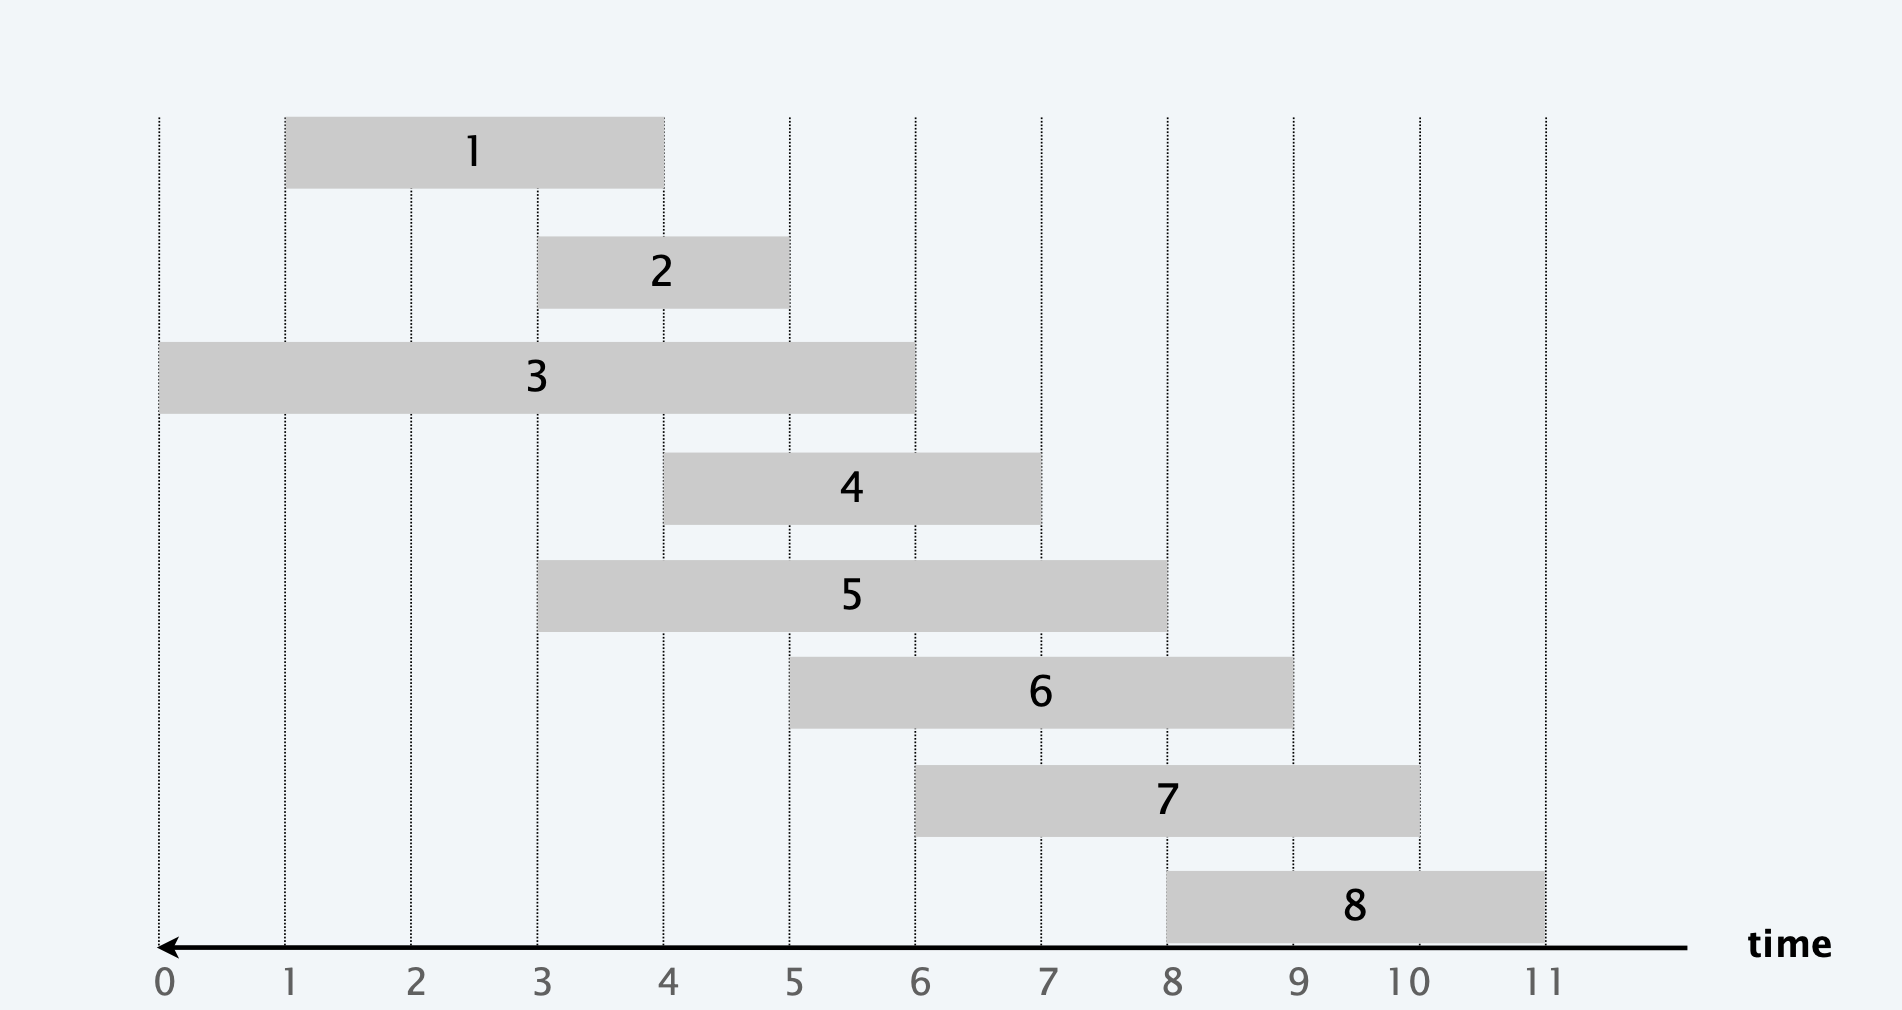
\includegraphics[width=0.7\textwidth ]{weighted}
    \caption{An instance for the weighted scheduling problem.}
\end{figure}

Example p(8) = 5 because the earliest compatible $j \in J$ with $j_{8}$ is $j_{5}$.More examples: p(7) = 3, p(2) = 0, ecc...\\\\
Now let's denote the OPT(j) as the value of optimal solution to the problem consisting, of job requests $1, 2, ..., j$. When dealing with dynamic programming, we have to build a formal definition of the recursion function, that defines the optimum at every step, but first we have to understand what happen at each iteration of the algorithm, the optimum can either:

\begin{itemize}

    \item {OPT selects job j}\\\\
          The algorithm then collect the profit $v_{j}$, then is locked out by all the incompatible jobs $\{ p(j) + 1, p(j) + 2, ..., j – 1 \}$, but must contain all the remain compatible jobs $\{1, 2, ..., p(j)\}$.

    \item {OPT does not select job j}\\\\
          Must include optimal solution to problem consisting of remaining compatible jobs $\{1, 2, ..., j – 1\}$.

          Merging all these informations we can build the recursion function:

          \[OPT(j) = \begin{cases} 0 \; if \; j = 0 \\ max\{vj \; + \; OPT(p(j)), OPT(j−1)\}  \end{cases}\]

\end{itemize}

Now for the implementation:

\begin{algorithm}[H]
    \SetAlgoLined
    \small
    \KwIn{$J$ set of jobs, each one with a $s_{j}$ start time, a finishing time $f_{j}$ and a reward $v_{j}$}
    \KwOut{$S$ containing the largest amount of compatible weighted jobs}
    \BlankLine

    $Js \leftarrow$ all the jobs sorted by increasing finishing time $f_{1} \leq f_{2} ... f_{j}$

    \BlankLine

    \For{i=0 to J.lenght }{
        \uIf{$i = 0$}{
            $M[i] = 0$ \;
        }
        \uElse{
            $M[i] = \emptyset$ \;

        }
    }

    \BlankLine

    $costMatrix = MComputeOpt(M,Js,J.last)$\;
    $return findSolution(M,currentJob)$

    \caption{DynamicWeightedInterval(J):}
\end{algorithm}

\begin{algorithm}[H]
    \SetAlgoLined
    \small
    \KwIn{$M$ Initialized Matrix containing all the reward,\; $J$ set of jobs, $currentJob$ to calculate the reward.}
    \KwOut{$M$ matrix containing all the computed values for each job}

    \BlankLine

    \uIf{$M[currentJob] = \emptyset$}{
    $M[currentJob] = max(currentJob.vj  + MComputeOpt(M,J,currentJob.pj), MComputeOpt(M,J,J[currentJob – 1]))$ \;
    }
    \uElse{
        $return \; M[currentJob]$ \;
    }

    \BlankLine

    \caption{MComputeOpt(M,J,currentJob):}
\end{algorithm}

\begin{algorithm}[H]
    \SetAlgoLined
    \small
    \KwIn{$M$ Initialized Matrix containing all the reward,\; $currentJob$ to calculate the reward.}
    \KwOut{$S$  containing the largest amount of compatible weighted jobs}
    \BlankLine

    \uIf{$currentJob = 0$}{
        return $\emptyset$ \;
    }
    \uElseIf{$currentJob.v_{j} + M[currentJob.p_{j}] > M[currentJob–1]$}{
    $return \{ j \} \cup FindSolution(M,currentJob.p_{j}).$
    }
    \uElse{
        $FindSolution(M,currentJob-1).$
    }

    \BlankLine

    \caption{findSolution(M,currentJob):}
\end{algorithm}

\begin{claim}
    The algorithm runs in $\mathcal{O}{(nlogn)}$
\end{claim}

\begin{proof}
    The recursive processes takes $\mathcal{O}{(n)}$ each, the most computational intensive operation is the sorting that takes $\mathcal{O}{(nlogn)}$, so overall we have $\mathcal{O}{(2n + nlogn)} \simeq$ $\mathcal{O}{(nlogn)} .$
\end{proof}

\subsection{Knapsack Problem}
Given N objects and a Knapsack(it's a backpack) with a capacity W, we have $\forall n \in N, \; w_{n} \geq 0 \; v_{n} \geq 0$, the goal is to fillup the Knapsack without exceeding it's capacity with the maximum value.

\begin{figure}[H]
    \centering
    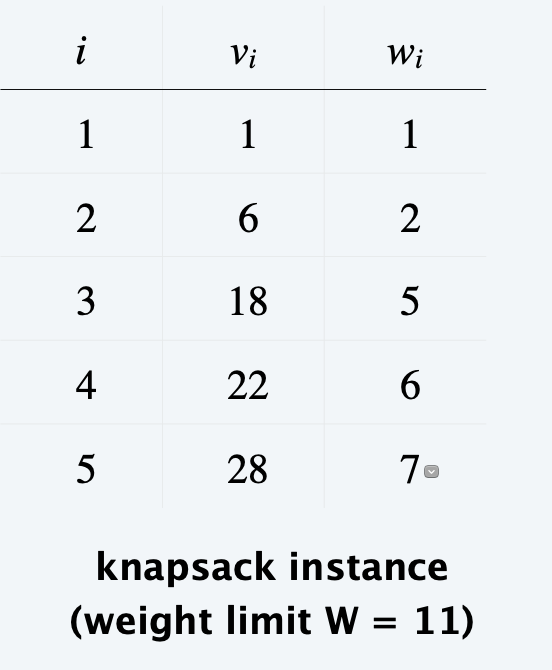
\includegraphics[width=0.2\textwidth ]{knapsack}
    \caption{An instance for the knapsack problem.}
\end{figure}

Example: $\{ 1, 2, 5 \}$ has value 35,  $\{ 3, 4 \}$ has value 40, $\{ 3, 5 \}$ has value 46 (but exceeds weight limit).

\begin{itemize}

    \item {Defining the Optimum}\\

          This time we have to take into account both the variation of the value of the content of the knapsack and the weight limit left:

          \[OPT(j) = \begin{cases} 0 \; if \; i = 0 \\ OPT(i-1,w) \; if \; w_{i} > w \\ max\{OPT(i−1,w),\; vi + OPT(i−1,w−w_{i})\} \; otherwise \}  \end{cases}\]

\end{itemize}

Now for the implementation:

\begin{algorithm}[H]
    \SetAlgoLined
    \small
    \KwIn{$N$ set of all the objects, each one with a $v_{j}$ value, and $w_{i}$ weight, $W$ the maximum capacity of the knapsack}
    \KwOut{$S$ containing the most valuable objects without exceeding w}
    \BlankLine

    \BlankLine

    \For{i=0 to w }{
        $M[0,wi] = 0$ \;
    }
    \For{j=1 to $N$ }{
        \For{k=1 to $W$ }{
            \uIf{$N[j].weight > k$}{
                $M[j,k] = M[j–1,k]$
            }
            \uElse{
                $M [ j, k ] =  max \{ M [ j – 1, k], vi + M [ j – 1, w – w_{j}] \}$.
            }
        }
    }


    \BlankLine
    return $M[n,W]$

    \caption{DynamicKnapsack(N,W):}
\end{algorithm}

\begin{figure}[H]
    \centering
    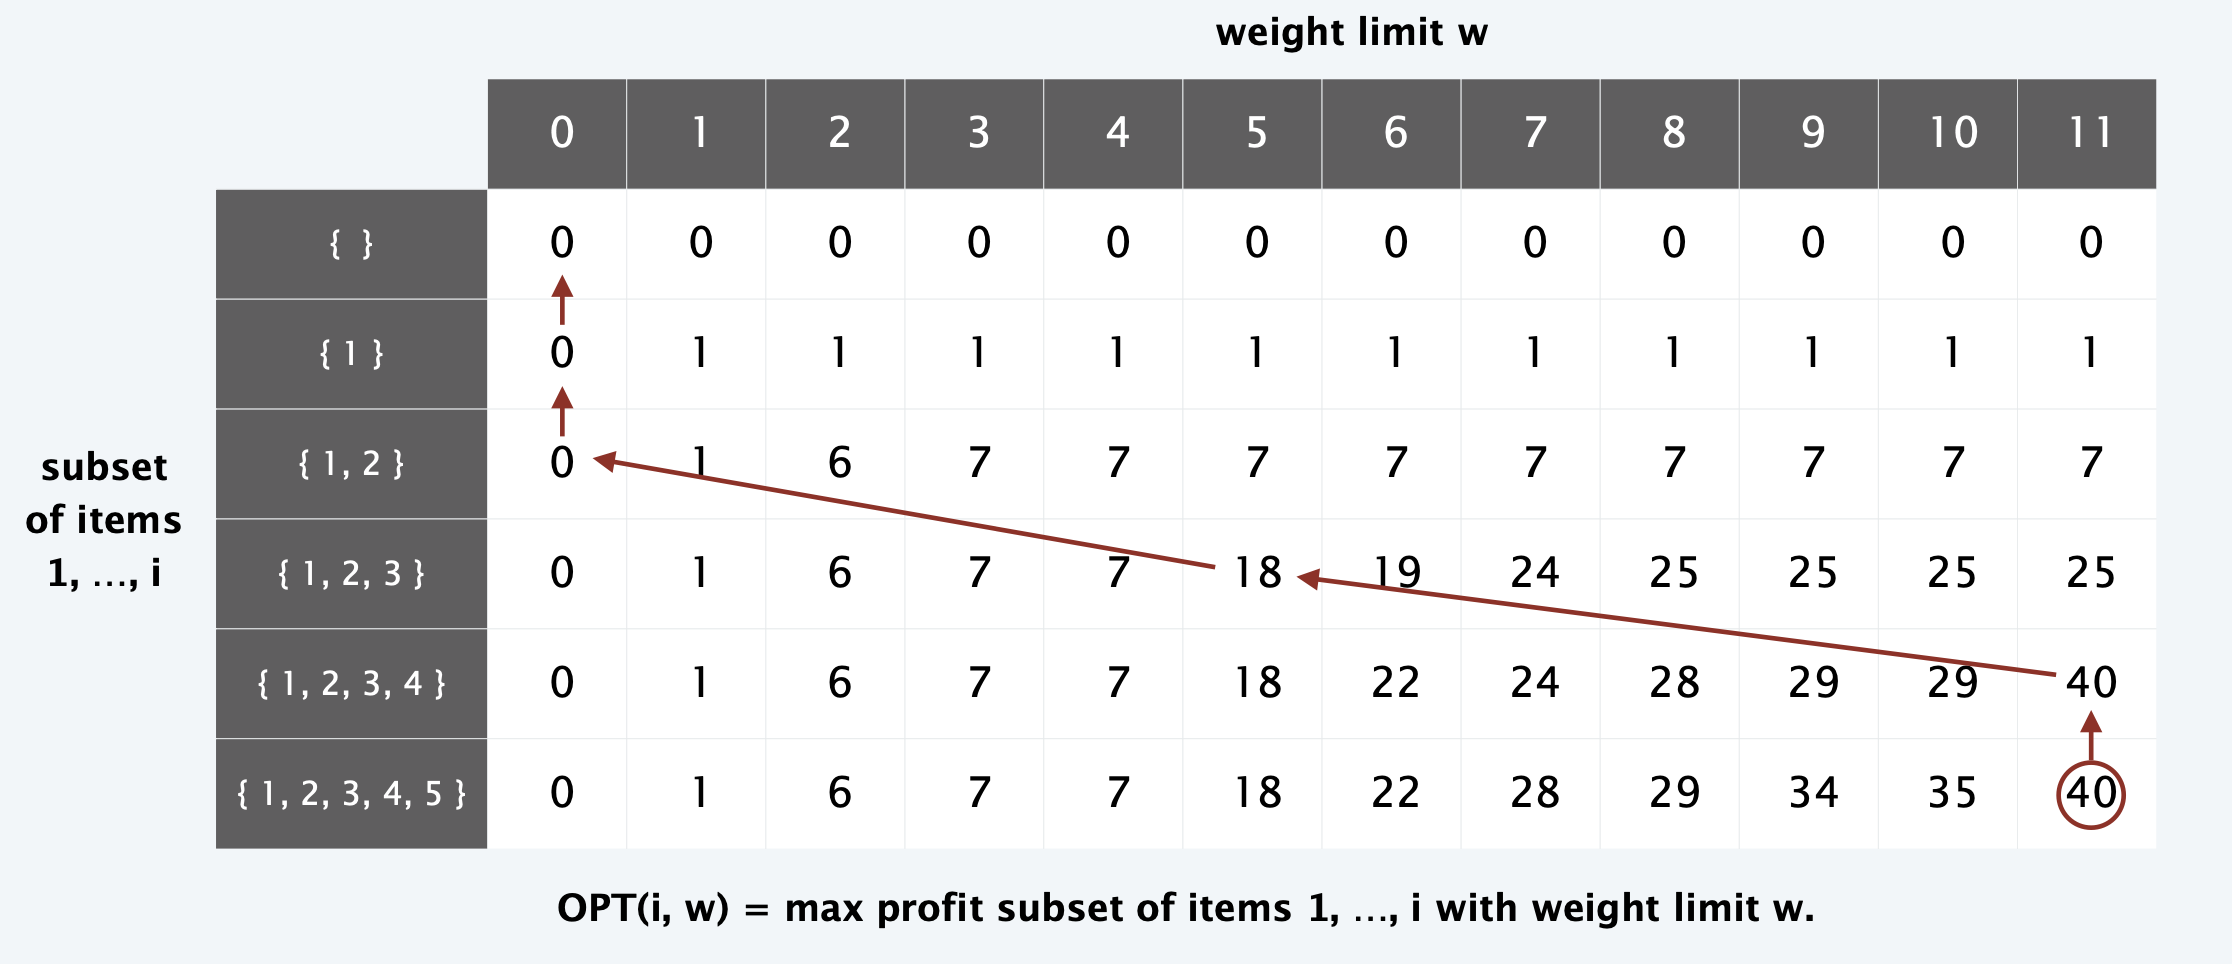
\includegraphics[width=0.8\textwidth ]{knapsack2}
    \caption{A table rapresenting the solution for the knapsack problem.}
\end{figure}

This algorithm is defined as pseudo-polinomial, because the execution time is proportional to the knapsack's W.\\

\begin{claim}
    The algorithm runs in Θ(nW)
\end{claim}

\begin{proof}
    We need to build a table of all the combinations of values and weight of dimension Θ(nW), $\forall n \in N$ so that's the execution time of the algorithm.
\end{proof}

\subsection{Sequence Alignment}
In this problem we want to measure the degree of similarity between two strings, first of all we have to make sure that the two strings have the same length, then we define a gap as $ \exists i \in s_{1} / s_2[i] = \emptyset$ or vice-versa, instead a mismatch as: $\exists i \in s_{1} / s_2[i] \neq s_{1}[i]$.

\begin{figure}[H]
    \centering
    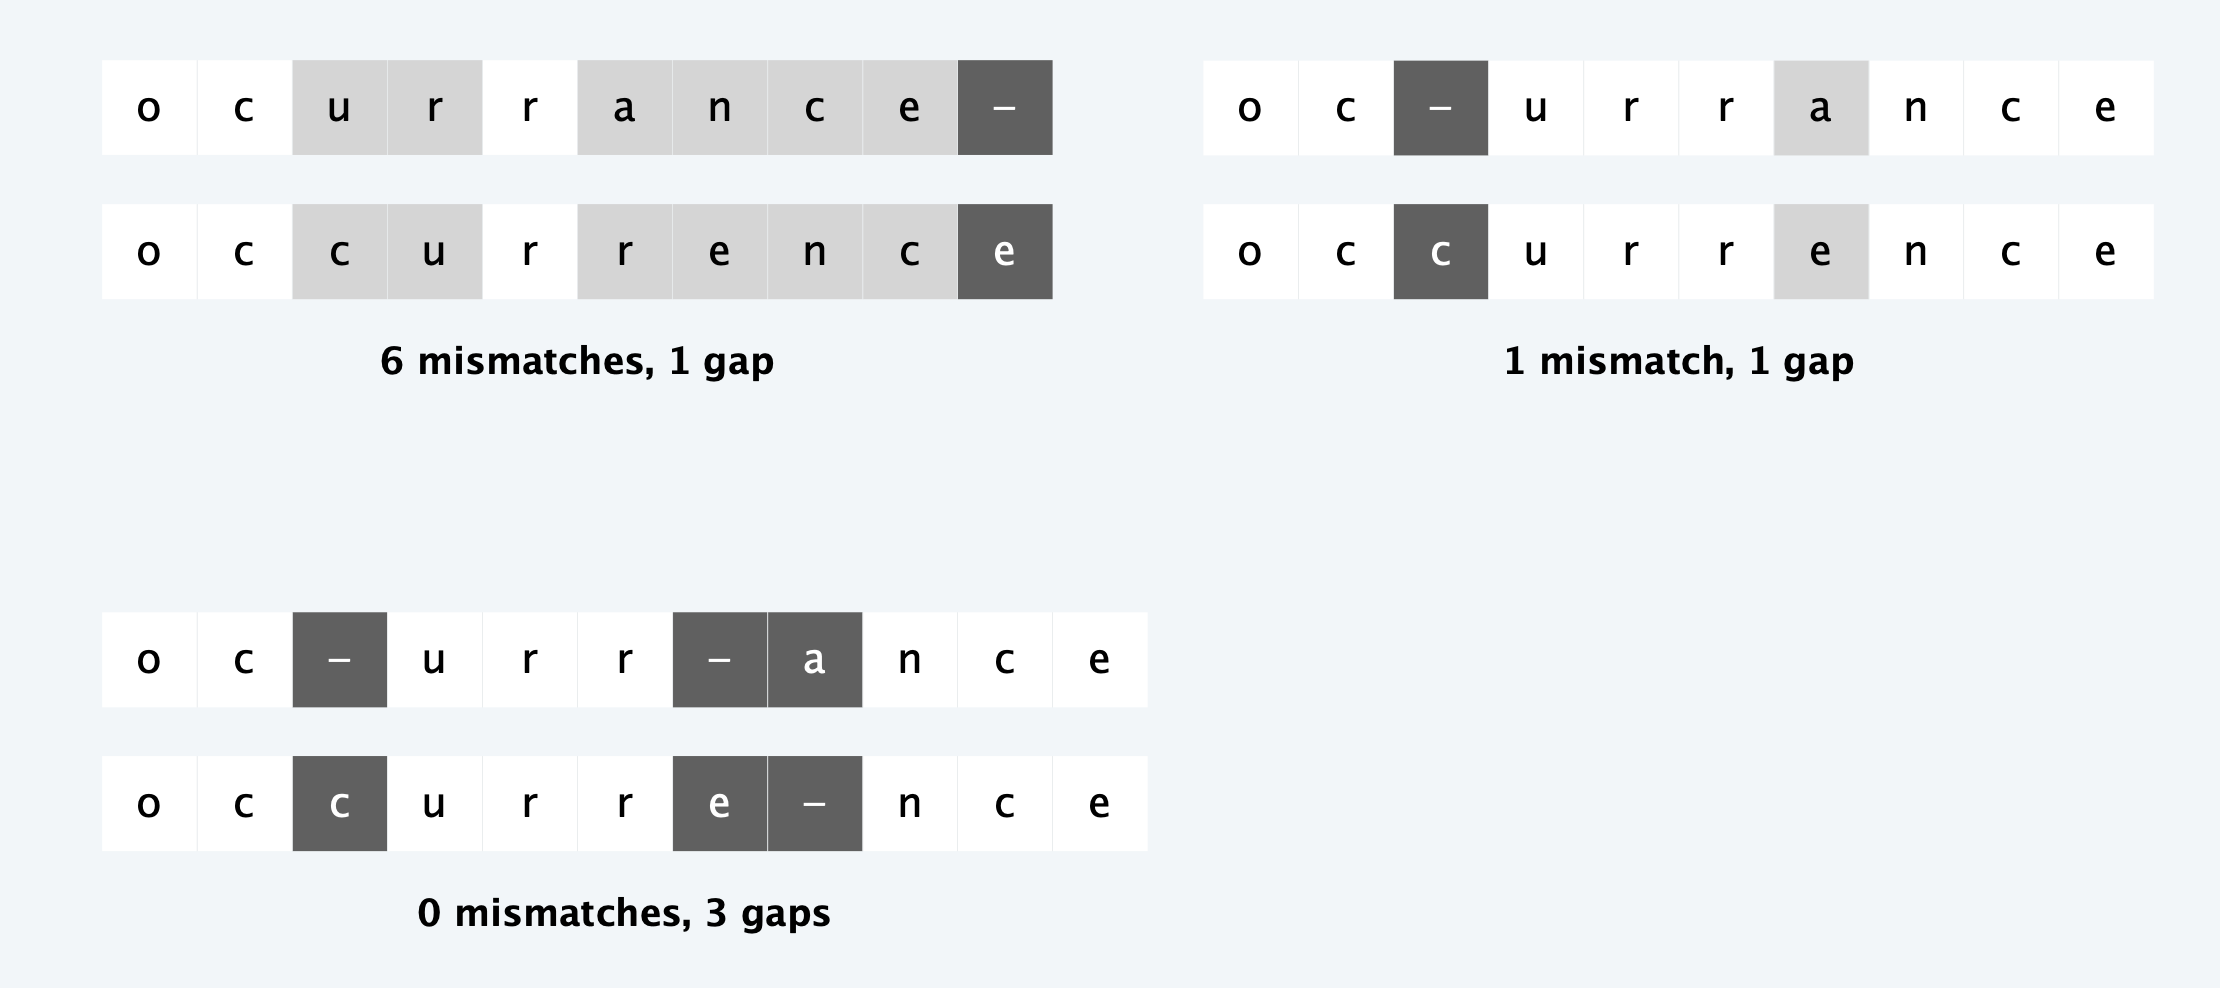
\includegraphics[width=0.6\textwidth ]{sequence}
    \caption{different approaches for the gap and occurrences in the sequence alignment problem.}
\end{figure}

To define a degree of similarities between two strings, we need a way to define a cost that rappresents the degree of difference between the strings, so for each gap we define a penalty $\delta$ and a mismatch penalty $\alpha_{p,q}$, so the total cost would be the sum of mismatch and gaps. Now we can re-formulate our problem as: given two strings $x_{1},x_{2}...x_{m}$ and $y_{1},y_{2}...y_{m}$, we want to find a minimum cost alignment defined as: a set of ordered pairs $x_{i} - y_{i}$ such that each item occurs in at most one pair and no crossings ($x_{i} – y_{j}$ and $x_{i'} – y_{j'}$ cross if $i < i '$, but $j > j '$).

\begin{figure}[H]
    \centering
    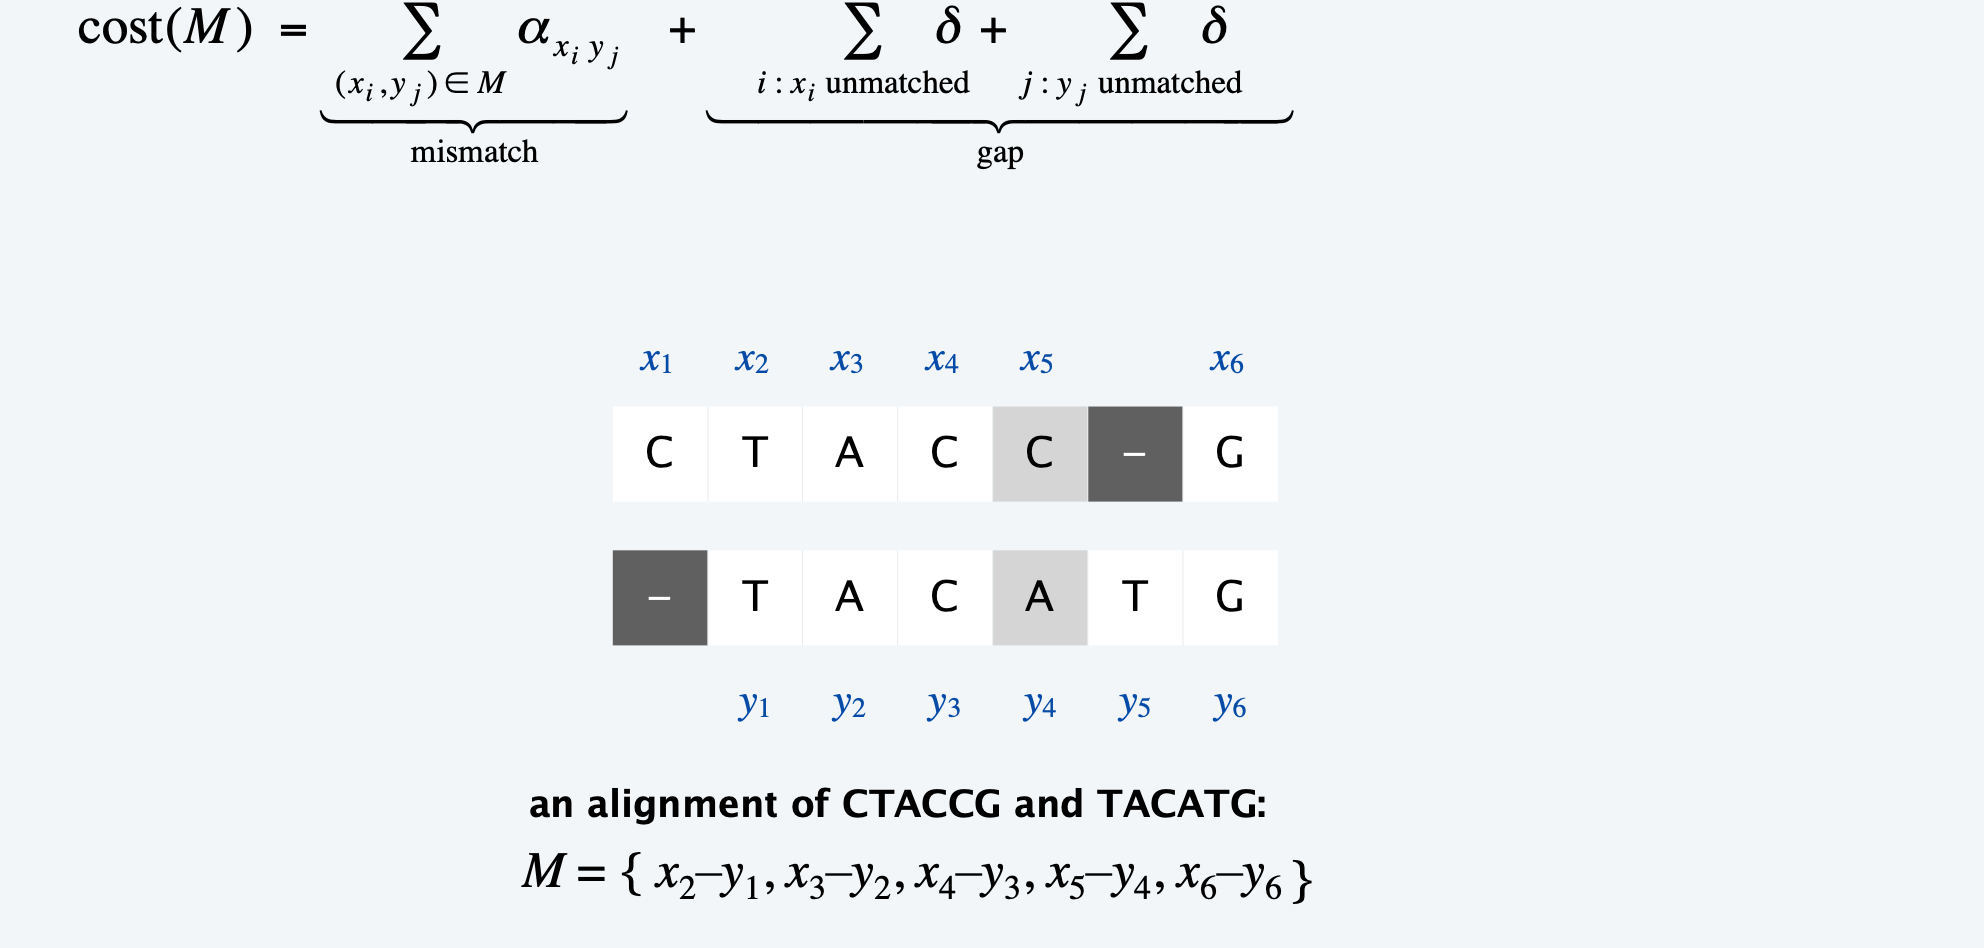
\includegraphics[width=0.6\textwidth ]{sequence2}
    \caption{Cost Definition.}
\end{figure}

Now, as usual we have to define the optimum as OPT(i, j) = min cost of aligning prefix in the two strings.

\begin{itemize}

    \item {Case 1: matches $x_{i} – y_{j}$.}\\
          Pay mismatch for $x_{i} – y_{j}$ + min cost of aligning $x_{1}, x_{2} ... x_{i–1}$ and $y_{1} ,y_{2} ... y_{j–1}$.

    \item {Case 2:OPT leaves $x_{i}$ unmatched.}\\
          Pay gap for $x_{i}$ + min cost of aligning $x_{1}, x_{2} ... x_{i–1}$ and $y_{1}, y_{2} ... y_{j}$.

    \item {Case 3:OPT leaves $y_{i}$ unmatched}\\
          Pay gap for $y_{j}$ + min cost of aligning $x{_1},x_{2} ... x{i}$ and $y_{1}, y_{2} ... y_{j}$.

\end{itemize}

\[OPT(j) = \begin{cases} i\delta \; if \; i = 0 \\ min \;otherwise \\ j\delta \; j=0 \}  \end{cases}\]
\[min=\begin{cases} \alpha _{x_{i} y_{j}} OPT(i−1, j-1) \\ \delta OPT(i−1, j) \\ \delta  O P T ( i , j − 1 )  \end{cases}\]


\begin{algorithm}[H]
    \SetAlgoLined
    \small
    \KwIn{$x$ String $y$ String}
    \KwOut{$S$ containing the minimum cost alignment.}

    \BlankLine

    \For{i=0 to x.lenght }{
        $M[i,0] = \delta i$ \;
    }

    \BlankLine

    \For{j=0 to y.lenght }{
        $M[j,0] = \delta j$ \;
    }

    \BlankLine

    \For{i=0 to x.lenght }{
        \For{j=0 to y.lenght }{
            $M[i,j] = min(\alpha[x_{i}, y_{j}] + M[i–1, j–1], \delta + M[i–1, j],\delta + M[i, j–1]) $\;
        }
    }

    \BlankLine
    return S = M[x.lenght][y.lenght]


    \caption{SequenceAllignment(x,y):}
\end{algorithm}

\begin{claim}
    The algorithm runs in Θ(mn) for two strings of length m and n.
\end{claim}

\begin{proof}
    We need to build a table of all the combinations of values and weight of dimension Θ(mn), same as 4.2
\end{proof}

\subsection{Bellman-Ford}
Algorithm for shortest path for graphs with negatives paths, unfortunately the Dikstra fails:

\begin{figure}[H]
    \centering
    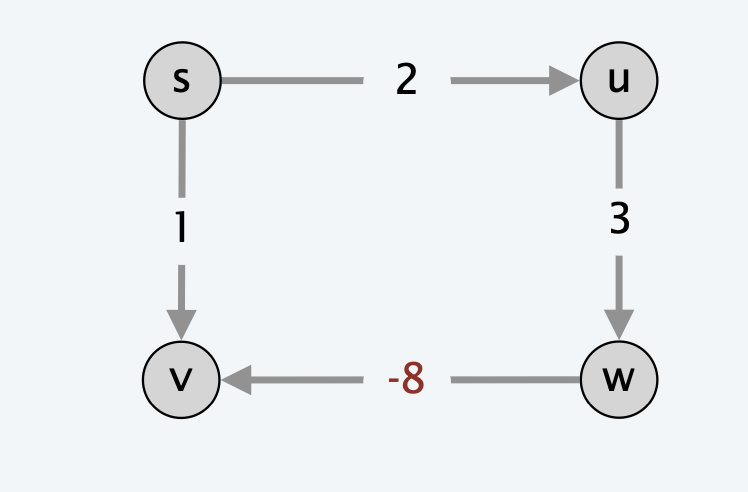
\includegraphics[width=0.3\textwidth ]{bellman}
    \caption{G=(V,E) with negative paths: the Dikstra algorithm will select c(s,v) = 1, ignoring the correct solution: c((s,u)+(u,w)+(w,v))=-3}
\end{figure}

\emph{Formal definition}:A negative path is a directed cycle such that the sum of its edge weights is negative.
\[ c(W) = \sum_{e \in W}^{} c_{e} < 0 \]

\begin{claim}
    If some path from v to t contains a negative cycle, then there does not exist a cheapest path from v to t.
\end{claim}\\

\begin{proof}
    If there exists such a cycle W, then can build a $v \rightarrow t$ path of arbitrarily negative weight by detouring around cycle as many times as desired.
\end{proof}\\

\begin{claim}
    If G has no negative cycles, then there exists a cheapest path from v to t that is simple (and has $\leq$ n – 1 edges).
\end{claim}

\begin{proof}
    Consider a cheapest $v\rightarrow t$ path P that uses the fewest number of edges, If P contains a cycle W, we can remove portion of P corresponding to W
    without increasing the cost.
\end{proof}\\

the OPT(i,v) = cost of shortest $v\rightarrow t$ path that uses i edges, with i $\leq |E|$.

\begin{itemize}

    \item {Case 1: Cheapest  $v\rightarrow t$ path uses $\leq$ i – 1 edges.}\\
          OPT(i, v) = OPT(i – 1, v)

    \item {Case 2:Cheapest  $v\rightarrow t$ path uses $\leq$ i edges.}\\
          if (v, w) is first edge, then OPT uses (v, w), and then selects best $w \rightarrow t$ path using $\leq$ i – 1 edges.


\end{itemize}

\[OPT(i,v) = \begin{cases} \infty \; if = 0  \\ min \; otherwise \end{cases}\]
\[min= \{ OPT(i-1,v),min_{(v,w) \in E} \{OPT(i−1, w)+c_{vw} \}\} \]

Implementation:

\begin{algorithm}[H]
    \SetAlgoLined
    \small
    \KwIn{$G$ directed graph with negative paths\; $s$ source node of the path, $t$ final node of the path.}
    \KwOut{$S$ containing the shortest path s $\leftarrow$ t}

    \BlankLine


    \BlankLine

    \caption{BellmanFord(G,s,t):}
\end{algorithm}

\begin{claim}
    The Bellman-Ford algorithm's cost is $\mathcal{O}{(nm)}$.
\end{claim}
\begin{proof}
    The successor graph cannot have a negative cycle,thus, following the successor pointers from s yields a directed path to t.\\
    Let $s = v_{1} \leftarrow v_{2} \leftarrow ... \leftarrow v_{k} = t$ be the nodes along this path P, upon termination, if successor(v) = w, we must have d(v) = d(w) + $c_{vw}$, putting it all together, we have:
    \[d(s) = d(t) + c(v_{1}, v_{2}) + c(v_{2}, v_{3}) + ... + c(v_{k–1}, v_{k})\]
\end{proof}


\clearpage

